\chapter{Caminos más cortos}

\index{camino más corto}

Encontrar un camino mínimo entre dos nodos de un grafo
es un problema importante que tiene muchas aplicaciones prácticas.
Por ejemplo, un problema natural relacionado a una red de calles
es calcular la distancia más corta de una ruta entre dos ciudades,
dadas las longitudes de las calles.

En un grafo no ponderado, la longitud de un camino es igual
a su número de aristas, y podemos simplemente usar la búsqueda en
anchura para encontrar un camino mínimo. Sin embargo, en este
capítulo nos centraremos en grafos ponderados, donde son necesarios
algoritmos más sofisticados.

\section{Algoritmo de Bellman--Ford}

\index{algoritmo de!Bellman--Ford}

El \key{algoritmo de Bellman--Ford}\footnote{Este algoritmo lleva
    el nombre de R. E. Bellman y L. R. Ford, quienes lo publicaron
    de manera independiente en 1958 y 1956, respectivamente
    \cite{bel58,for56a}.}
encuentra los caminos más cortos desde un nodo inicial a todos los
nodos del grafo. El algoritmo puede procesar todo tipo de grafo,
dado que no contenga ciclos con longitud negativa. Si es así, el
algoritmo puede detectarlo.

El algoritmo mantiene una lista de distancias desde el nodo inicial
a todos los nodos del grafo. Inicialmente, la distancia a sí mismo
es 0, y la distancia a todos los otros nodos es infinita. El
algoritmo reduce las distancias encontrando aristas que acorten
los caminos hasta que no sea posible reducir ninguna distancia.

\subsubsection{Ejemplo}

Veamos cómo funciona el algoritmo de Bellman--Ford
en el siguiente grafo:

\begin{center}
    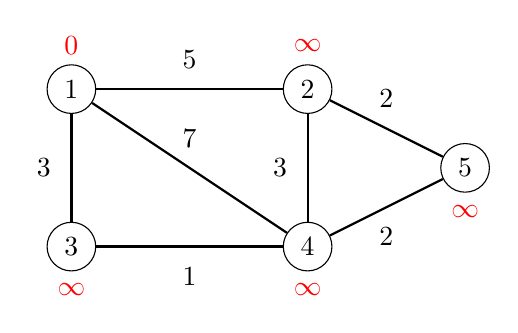
\begin{tikzpicture}
        \node[draw, circle] (1) at (1,3) {1};
        \node[draw, circle] (2) at (4,3) {2};
        \node[draw, circle] (3) at (1,1) {3};
        \node[draw, circle] (4) at (4,1) {4};
        \node[draw, circle] (5) at (6,2) {5};
        \node[color=red] at (1,3+0.55) {$0$};
        \node[color=red] at (4,3+0.55) {$\infty$};
        \node[color=red] at (1,1-0.55) {$\infty$};
        \node[color=red] at (4,1-0.55) {$\infty$};
        \node[color=red] at (6,2-0.55) {$\infty$};
        \path[draw,thick,-] (1) -- node[font=\small,label=above:5] {} (2);
        \path[draw,thick,-] (1) -- node[font=\small,label=left:3] {} (3);
        \path[draw,thick,-] (3) -- node[font=\small,label=below:1] {} (4);
        \path[draw,thick,-] (2) -- node[font=\small,label=left:3] {} (4);
        \path[draw,thick,-] (2) -- node[font=\small,label=above:2] {} (5);
        \path[draw,thick,-] (4) -- node[font=\small,label=below:2] {} (5);
        \path[draw,thick,-] (1) -- node[font=\small,label=above:7] {} (4);
    \end{tikzpicture}
\end{center}

Cada nodo del grafo es asignado una distancia. El algoritmo
busca aristas que reduzcan distancias. Primero, todas las aristas
del nodo 1 reducen distancias:
\begin{center}
    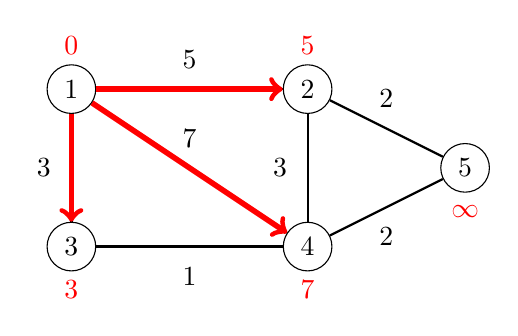
\begin{tikzpicture}
        \node[draw, circle] (1) at (1,3) {1};
        \node[draw, circle] (2) at (4,3) {2};
        \node[draw, circle] (3) at (1,1) {3};
        \node[draw, circle] (4) at (4,1) {4};
        \node[draw, circle] (5) at (6,2) {5};
        \node[color=red] at (1,3+0.55) {$0$};
        \node[color=red] at (4,3+0.55) {$5$};
        \node[color=red] at (1,1-0.55) {$3$};
        \node[color=red] at (4,1-0.55) {$7$};
        \node[color=red] at (6,2-0.55) {$\infty$};
        \path[draw,thick,-] (1) -- node[font=\small,label=above:5] {} (2);
        \path[draw,thick,-] (1) -- node[font=\small,label=left:3] {} (3);
        \path[draw,thick,-] (3) -- node[font=\small,label=below:1] {} (4);
        \path[draw,thick,-] (2) -- node[font=\small,label=left:3] {} (4);
        \path[draw,thick,-] (2) -- node[font=\small,label=above:2] {} (5);
        \path[draw,thick,-] (4) -- node[font=\small,label=below:2] {} (5);
        \path[draw,thick,-] (1) -- node[font=\small,label=above:7] {} (4);

        \path[draw=red,thick,->,line width=2pt] (1) -- (2);
        \path[draw=red,thick,->,line width=2pt] (1) -- (3);
        \path[draw=red,thick,->,line width=2pt] (1) -- (4);
    \end{tikzpicture}
\end{center}

Luego, las aristas $2 \rightarrow 5$ y $3 \rightarrow 4$
reducen distancias:
\begin{center}
    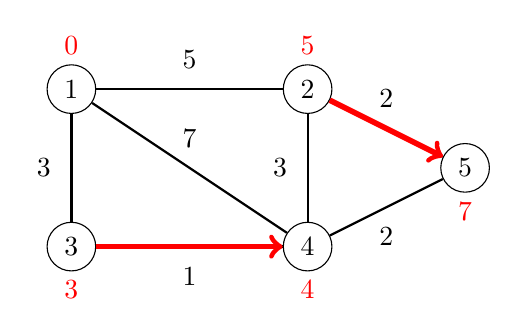
\begin{tikzpicture}
        \node[draw, circle] (1) at (1,3) {1};
        \node[draw, circle] (2) at (4,3) {2};
        \node[draw, circle] (3) at (1,1) {3};
        \node[draw, circle] (4) at (4,1) {4};
        \node[draw, circle] (5) at (6,2) {5};
        \node[color=red] at (1,3+0.55) {$0$};
        \node[color=red] at (4,3+0.55) {$5$};
        \node[color=red] at (1,1-0.55) {$3$};
        \node[color=red] at (4,1-0.55) {$4$};
        \node[color=red] at (6,2-0.55) {$7$};
        \path[draw,thick,-] (1) -- node[font=\small,label=above:5] {} (2);
        \path[draw,thick,-] (1) -- node[font=\small,label=left:3] {} (3);
        \path[draw,thick,-] (3) -- node[font=\small,label=below:1] {} (4);
        \path[draw,thick,-] (2) -- node[font=\small,label=left:3] {} (4);
        \path[draw,thick,-] (2) -- node[font=\small,label=above:2] {} (5);
        \path[draw,thick,-] (4) -- node[font=\small,label=below:2] {} (5);
        \path[draw,thick,-] (1) -- node[font=\small,label=above:7] {} (4);

        \path[draw=red,thick,->,line width=2pt] (2) -- (5);
        \path[draw=red,thick,->,line width=2pt] (3) -- (4);
    \end{tikzpicture}
\end{center}
Finalmente, hay un cambio más:
\begin{center}
    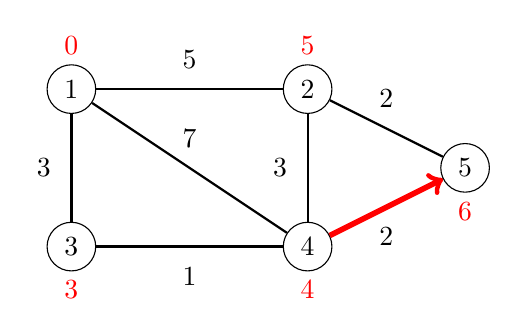
\begin{tikzpicture}
        \node[draw, circle] (1) at (1,3) {1};
        \node[draw, circle] (2) at (4,3) {2};
        \node[draw, circle] (3) at (1,1) {3};
        \node[draw, circle] (4) at (4,1) {4};
        \node[draw, circle] (5) at (6,2) {5};
        \node[color=red] at (1,3+0.55) {$0$};
        \node[color=red] at (4,3+0.55) {$5$};
        \node[color=red] at (1,1-0.55) {$3$};
        \node[color=red] at (4,1-0.55) {$4$};
        \node[color=red] at (6,2-0.55) {$6$};
        \path[draw,thick,-] (1) -- node[font=\small,label=above:5] {} (2);
        \path[draw,thick,-] (1) -- node[font=\small,label=left:3] {} (3);
        \path[draw,thick,-] (3) -- node[font=\small,label=below:1] {} (4);
        \path[draw,thick,-] (2) -- node[font=\small,label=left:3] {} (4);
        \path[draw,thick,-] (2) -- node[font=\small,label=above:2] {} (5);
        \path[draw,thick,-] (4) -- node[font=\small,label=below:2] {} (5);
        \path[draw,thick,-] (1) -- node[font=\small,label=above:7] {} (4);

        \path[draw=red,thick,->,line width=2pt] (4) -- (5);
    \end{tikzpicture}
\end{center}

Finalmente, ningún nodo puede reducir su distancia.
Esto significa que las distancias son finales, y hemos
calculado las distancias más cortas desde el nodo inicial
a todos los nodos del grafo.

Por ejemplo, la distancia más corta 3 del nodo 1
al nodo 5 corresponde al siguiente camino:

\begin{center}
    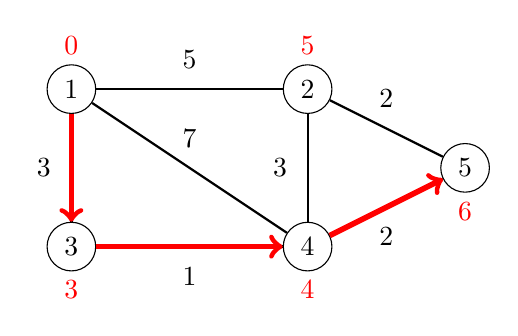
\begin{tikzpicture}
        \node[draw, circle] (1) at (1,3) {1};
        \node[draw, circle] (2) at (4,3) {2};
        \node[draw, circle] (3) at (1,1) {3};
        \node[draw, circle] (4) at (4,1) {4};
        \node[draw, circle] (5) at (6,2) {5};
        \node[color=red] at (1,3+0.55) {$0$};
        \node[color=red] at (4,3+0.55) {$5$};
        \node[color=red] at (1,1-0.55) {$3$};
        \node[color=red] at (4,1-0.55) {$4$};
        \node[color=red] at (6,2-0.55) {$6$};
        \path[draw,thick,-] (1) -- node[font=\small,label=above:5] {} (2);
        \path[draw,thick,-] (1) -- node[font=\small,label=left:3] {} (3);
        \path[draw,thick,-] (3) -- node[font=\small,label=below:1] {} (4);
        \path[draw,thick,-] (2) -- node[font=\small,label=left:3] {} (4);
        \path[draw,thick,-] (2) -- node[font=\small,label=above:2] {} (5);
        \path[draw,thick,-] (4) -- node[font=\small,label=below:2] {} (5);
        \path[draw,thick,-] (1) -- node[font=\small,label=above:7] {} (4);

        \path[draw=red,thick,->,line width=2pt] (1) -- (3);
        \path[draw=red,thick,->,line width=2pt] (3) -- (4);
        \path[draw=red,thick,->,line width=2pt] (4) -- (5);
    \end{tikzpicture}
\end{center}

\subsubsection{Implementación}

La siguiente implementación del algoritmo de Bellman--Ford
determina las distancias mínimas de un nodo $x$ a todos los
nodos del grafo. El código asume que el grafo está almacenado
en una lista de \texttt{aristas}, que consiste de tuplas
en forma $(a, b, p)$, significando que hay una arista del
nodo $a$ al nodo $b$ con peso $p$.

El algoritmo consiste en $n-1$ rondas, y en cada ronda
este visita todas las aristas del grafo e intenta reducir las
distancias. El algoritmo construye un arreglo \texttt{distancia}
que contendrá las distancias desde $x$ a todos los nodos del grafo.
La constante \texttt{INF} denota una distancia infinita.

\begin{lstlisting}
for (int i = 1; i <= n; i++) distancia[i] = INF;
distancia[x] = 0;
for (int i = 1; i <= n-1; i++) {
    for (auto arista : aristas) {
        int a, b, p;
        tie(a, b, p) = arista;
        distancia[b] = min(distancia[b], distancia[a] + p);
    }
}
\end{lstlisting}

La complejidad temporal del algoritmo es $O(nm)$,
porque consiste en $n-1$ rondas e itera a través de todas
las $m$ aristas durante una ronda. Si no hay ciclos negativos
en el grafo, todas las distancias son finales luego de $n-1$ rondas,
porque cada camino mínimo puede contener como mucho $n-1$ aristas.

En la práctica, las distancias finales usualmente pueden encontrarse
más rápido que en $n-1$ rondas. Por lo tanto, una manera posible de
optimizar el algoritmo es frenarlo si ninguna distancia pudo
reducirse durante una ronda.

\subsubsection{Ciclos negativos}

\index{ciclo negativo}

El algoritmo de Bellman--Ford también puede utilizarse para
revisar si el grafo contiene un ciclo con longitud negativa.
Por ejemplo, el grafo.

\begin{center}
    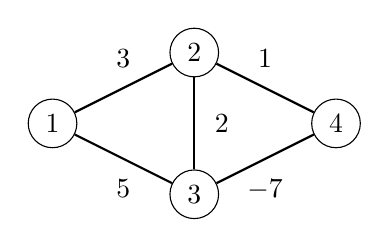
\begin{tikzpicture}[scale=0.9]
        \node[draw, circle] (1) at (0,0) {$1$};
        \node[draw, circle] (2) at (2,1) {$2$};
        \node[draw, circle] (3) at (2,-1) {$3$};
        \node[draw, circle] (4) at (4,0) {$4$};

        \path[draw,thick,-] (1) -- node[font=\small,label=above:$3$] {} (2);
        \path[draw,thick,-] (2) -- node[font=\small,label=above:$1$] {} (4);
        \path[draw,thick,-] (1) -- node[font=\small,label=below:$5$] {} (3);
        \path[draw,thick,-] (3) -- node[font=\small,label=below:$-7$] {} (4);
        \path[draw,thick,-] (2) -- node[font=\small,label=right:$2$] {} (3);
    \end{tikzpicture}
\end{center}
\noindent

contiene un ciclo negativo
$2 \rightarrow 3 \rightarrow 4 \rightarrow 2$
con longitud $-4$.

Si el grafo contiene un ciclo negativo, podemos acortar
infinitamente cualquier camino que contenga el ciclo si
repetimos el ciclo una y otra vez. Por lo tanto, el concepto
de un camino mínimo no tiene sentido en esta situación.

Un ciclo negativo puede ser detectado utilizando el algoritmo
de Bellman--Ford ejecutándolo por $n$ rondas. Si la última ronda
reduce alguna distancia, entonces el grafo contiene un ciclo negativo.
Ten en cuenta que este algoritmo puede utilizarse para buscar
un ciclo negativo en todo el grafo independientemente del nodo inicial.

\subsubsection{Algoritmo SPFA}

\index{algoritmo!SPFA}

El \key{algoritmo SPFA}\footnote{De \textit{shortest path faster algorithm},
    ``algoritmo más rápido de camino mínimo'' \cite{fan94}} es una variante
del algoritmo de Bellman--Ford que es, a menudo, más eficiente que el
algoritmo original. El algoritmo SPFA no visita todos los nodos en cada
ronda, sino que elige los nodos a examinar de una forma más inteligente.

El algoritmo mantiene una cola de nodos que tal vez puedan ser
utilizados para reducir las distancias. Primero, el algoritmo añade
el nodo inicial $x$ a la cola. Luego, el algoritmo siempre procesa
el primer nodo en la cola, y cuando una arista $a \rightarrow b$
reduce una distancia, el nodo $b$ es añadido a la cola.

La eficiencia del algoritmo SPFA depende de la estructura del grafo:
normalmente el algoritmo es más eficiente, pero su complejidad
temporal en el peor caso sigue siendo $O(nm)$, y es posible crear
entradas que hagan el algoritmo tan lento como el original de
Bellman--Ford.

\section{Algoritmo de Dijkstra}

\index{algoritmo de!Dijkstra}

El \key{algoritmo de Dijkstra}\footnote{E. W. Dijkstra (pronunciado
    \textit{daik-stra}) publicó el algoritmo en 1959 \cite{dij59};
    sin embargo, su publicación original no menciona cómo implementar
    el algoritmo eficientemente.} encuentra caminos mínimos desde el
nodo inicial a todos los otros nodos del grafo, tal como el algoritmo
de Bellman--Ford. El beneficio del algoritmo de Dijkstra es su eficiencia.
De todas formas, el algoritmo requiere que no haya aristas de peso
negativo en el grafo.

Así como el de Bellman--Ford, el algoritmo de Dijkstra
mantiene distancias al resto de los nodos y las reduce durante la
búsqueda. Este algoritmo es eficiente porque solamente procesa
cada nodo en el grafo una vez, tomando en cuenta el hecho de que
no hay aristas negativas.

\subsubsection{Ejemplo}

Veamos cómo funciona el algoritmo de Dijkstra en el siguiente
grafo, cuando el nodo inicial es el nodo 1:
\begin{center}
    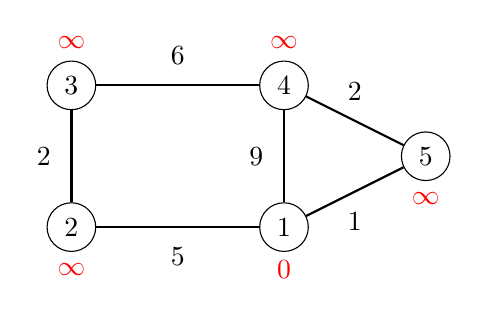
\begin{tikzpicture}[scale=0.9]
        \node[draw, circle] (1) at (1,3) {3};
        \node[draw, circle] (2) at (4,3) {4};
        \node[draw, circle] (3) at (1,1) {2};
        \node[draw, circle] (4) at (4,1) {1};
        \node[draw, circle] (5) at (6,2) {5};

        \node[color=red] at (1,3+0.6) {$\infty$};
        \node[color=red] at (4,3+0.6) {$\infty$};
        \node[color=red] at (1,1-0.6) {$\infty$};
        \node[color=red] at (4,1-0.6) {$0$};
        \node[color=red] at (6,2-0.6) {$\infty$};

        \path[draw,thick,-] (1) -- node[font=\small,label=above:6] {} (2);
        \path[draw,thick,-] (1) -- node[font=\small,label=left:2] {} (3);
        \path[draw,thick,-] (3) -- node[font=\small,label=below:5] {} (4);
        \path[draw,thick,-] (2) -- node[font=\small,label=left:9] {} (4);
        \path[draw,thick,-] (2) -- node[font=\small,label=above:2] {} (5);
        \path[draw,thick,-] (4) -- node[font=\small,label=below:1] {} (5);
    \end{tikzpicture}
\end{center}

Como en el algoritmo de Bellman--Ford, inicialmente la distancia
al nodo inicial es 0 y la distancia a todos los otros nodos es infinita.

En cada paso, el algoritmo de Dijkstra elige un nodo que no haya
sido procesado todavía y cuya distancia sea lo más pequeña posible.
El primer nodo tal es el nodo 1 con distancia 0.

Cuando un nodo es elegido, el algoritmo visita todas las aristas
que comienzan en el nodo y reduce distancias utilizándolas:
\begin{center}
    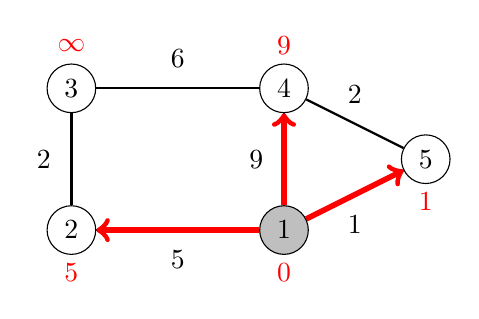
\begin{tikzpicture}[scale=0.9]
        \node[draw, circle] (1) at (1,3) {3};
        \node[draw, circle] (2) at (4,3) {4};
        \node[draw, circle] (3) at (1,1) {2};
        \node[draw, circle, fill=lightgray] (4) at (4,1) {1};
        \node[draw, circle] (5) at (6,2) {5};

        \node[color=red] at (1,3+0.6) {$\infty$};
        \node[color=red] at (4,3+0.6) {$9$};
        \node[color=red] at (1,1-0.6) {$5$};
        \node[color=red] at (4,1-0.6) {$0$};
        \node[color=red] at (6,2-0.6) {$1$};

        \path[draw,thick,-] (1) -- node[font=\small,label=above:6] {} (2);
        \path[draw,thick,-] (1) -- node[font=\small,label=left:2] {} (3);
        \path[draw,thick,-] (3) -- node[font=\small,label=below:5] {} (4);
        \path[draw,thick,-] (2) -- node[font=\small,label=left:9] {} (4);
        \path[draw,thick,-] (2) -- node[font=\small,label=above:2] {} (5);
        \path[draw,thick,-] (4) -- node[font=\small,label=below:1] {} (5);

        \path[draw=red,thick,->,line width=2pt] (4) -- (2);
        \path[draw=red,thick,->,line width=2pt] (4) -- (3);
        \path[draw=red,thick,->,line width=2pt] (4) -- (5);
    \end{tikzpicture}
\end{center}

En este caso, las aristas del nodo 1 reducen las distancias de los
nodos 2, 4, y 5, cuyas distancias son ahora 5, 9, y 1.

El siguiente nodo a procesar es el nodo 5 con distancia 1.
Esto reduce la distancia al nodo 4 de 9 a 3:
\begin{center}
    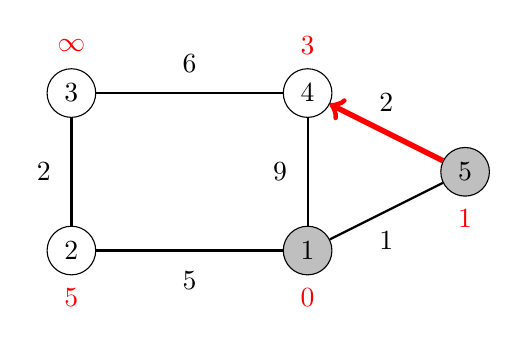
\begin{tikzpicture}
        \node[draw, circle] (1) at (1,3) {3};
        \node[draw, circle] (2) at (4,3) {4};
        \node[draw, circle] (3) at (1,1) {2};
        \node[draw, circle, fill=lightgray] (4) at (4,1) {1};
        \node[draw, circle, fill=lightgray] (5) at (6,2) {5};

        \node[color=red] at (1,3+0.6) {$\infty$};
        \node[color=red] at (4,3+0.6) {$3$};
        \node[color=red] at (1,1-0.6) {$5$};
        \node[color=red] at (4,1-0.6) {$0$};
        \node[color=red] at (6,2-0.6) {$1$};

        \path[draw,thick,-] (1) -- node[font=\small,label=above:6] {} (2);
        \path[draw,thick,-] (1) -- node[font=\small,label=left:2] {} (3);
        \path[draw,thick,-] (3) -- node[font=\small,label=below:5] {} (4);
        \path[draw,thick,-] (2) -- node[font=\small,label=left:9] {} (4);
        \path[draw,thick,-] (2) -- node[font=\small,label=above:2] {} (5);
        \path[draw,thick,-] (4) -- node[font=\small,label=below:1] {} (5);

        \path[draw=red,thick,->,line width=2pt] (5) -- (2);
    \end{tikzpicture}
\end{center}
Ahora, el siguiente nodo es 4, que reduce la distancia del nodo 3 a 9:
\begin{center}
    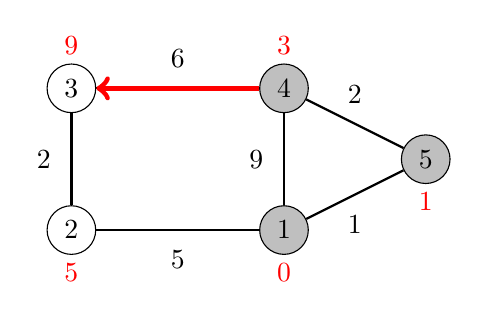
\begin{tikzpicture}[scale=0.9]
        \node[draw, circle] (1) at (1,3) {3};
        \node[draw, circle, fill=lightgray] (2) at (4,3) {4};
        \node[draw, circle] (3) at (1,1) {2};
        \node[draw, circle, fill=lightgray] (4) at (4,1) {1};
        \node[draw, circle, fill=lightgray] (5) at (6,2) {5};

        \node[color=red] at (1,3+0.6) {$9$};
        \node[color=red] at (4,3+0.6) {$3$};
        \node[color=red] at (1,1-0.6) {$5$};
        \node[color=red] at (4,1-0.6) {$0$};
        \node[color=red] at (6,2-0.6) {$1$};

        \path[draw,thick,-] (1) -- node[font=\small,label=above:6] {} (2);
        \path[draw,thick,-] (1) -- node[font=\small,label=left:2] {} (3);
        \path[draw,thick,-] (3) -- node[font=\small,label=below:5] {} (4);
        \path[draw,thick,-] (2) -- node[font=\small,label=left:9] {} (4);
        \path[draw,thick,-] (2) -- node[font=\small,label=above:2] {} (5);
        \path[draw,thick,-] (4) -- node[font=\small,label=below:1] {} (5);

        \path[draw=red,thick,->,line width=2pt] (2) -- (1);
    \end{tikzpicture}
\end{center}

Una propiedad notable del algoritmo de Dijkstra es que siempre que
un nodo es elegido, su distancia es final. Por ejemplo, en este punto
del algoritmo, las distancias 0, 1, y 3 son las distancias finales
a los nodos 1, 5, y 4.

Luego de esto, el algoritmo procesa los dos nodos restantes,
y las distancias finales son las siguientes:
\begin{center}
    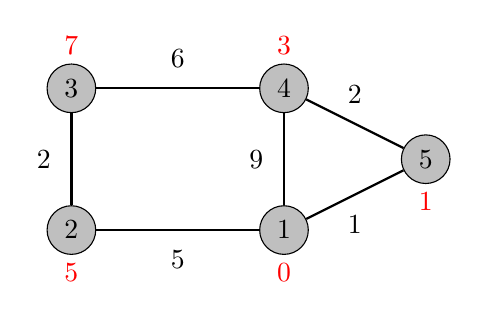
\begin{tikzpicture}[scale=0.9]
        \node[draw, circle, fill=lightgray] (1) at (1,3) {3};
        \node[draw, circle, fill=lightgray] (2) at (4,3) {4};
        \node[draw, circle, fill=lightgray] (3) at (1,1) {2};
        \node[draw, circle, fill=lightgray] (4) at (4,1) {1};
        \node[draw, circle, fill=lightgray] (5) at (6,2) {5};

        \node[color=red] at (1,3+0.6) {$7$};
        \node[color=red] at (4,3+0.6) {$3$};
        \node[color=red] at (1,1-0.6) {$5$};
        \node[color=red] at (4,1-0.6) {$0$};
        \node[color=red] at (6,2-0.6) {$1$};

        \path[draw,thick,-] (1) -- node[font=\small,label=above:6] {} (2);
        \path[draw,thick,-] (1) -- node[font=\small,label=left:2] {} (3);
        \path[draw,thick,-] (3) -- node[font=\small,label=below:5] {} (4);
        \path[draw,thick,-] (2) -- node[font=\small,label=left:9] {} (4);
        \path[draw,thick,-] (2) -- node[font=\small,label=above:2] {} (5);
        \path[draw,thick,-] (4) -- node[font=\small,label=below:1] {} (5);
    \end{tikzpicture}
\end{center}

\subsubsection{Aristas negativas}

La eficiencia del algoritmo de Dijkstra yace en el hecho de que
el grafo no contiene aristas negativas. Si hay una arista negativa,
el algoritmo puede dar resultados incorrectos. Por ejemplo,
considera el siguiente grafo:
\begin{center}
    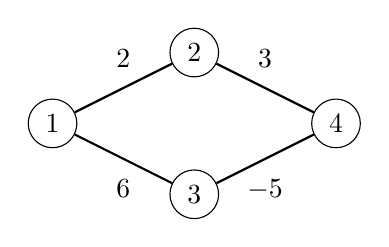
\begin{tikzpicture}[scale=0.9]
        \node[draw, circle] (1) at (0,0) {$1$};
        \node[draw, circle] (2) at (2,1) {$2$};
        \node[draw, circle] (3) at (2,-1) {$3$};
        \node[draw, circle] (4) at (4,0) {$4$};

        \path[draw,thick,-] (1) -- node[font=\small,label=above:2] {} (2);
        \path[draw,thick,-] (2) -- node[font=\small,label=above:3] {} (4);
        \path[draw,thick,-] (1) -- node[font=\small,label=below:6] {} (3);
        \path[draw,thick,-] (3) -- node[font=\small,label=below:$-5$] {} (4);
    \end{tikzpicture}
\end{center}
\noindent

El camino mínimo del nodo 1 al nodo 4 es $1 \rightarrow 3 \rightarrow 4$
con una longitud de 1. Sin embargo, el algoritmo de Dijkstra encuentra
el camino $1 \rightarrow 2 \rightarrow 4$ siguiendo las aristas de
peso mínimo. El algoritmo no toma en cuenta que en el otro camino, el
peso $-5$ compensa por el previo gran peso $6$.

\subsubsection{Implementación}

La siguiente implementación del algoritmo de Dijkstra calcula
las distancias mínimas de un nodo $x$ a todos los otros nodos del grafo.
El grafo está almacenado como listas de adyacencia tal que
\texttt{adj[$a$]} contiene un par $(b,p)$ siempre y cuando existe una
arista del nodo $a$ al nodo $b$ con peso $p$.

Una implementación eficiente del algoritmo de Dijkstra requiere
que sea posible encontrar eficientemente el nodo a mínima distancia
que no haya sido procesado. Una estructura de datos apropiada para
esto es una cola de prioridad que contenga los nodos ordenados
por distancia. Utilizando una cola de prioridad, el siguiente nodo
a procesar se puede acceder en tiempo logarítmico.

En el siguiente código, la cola de prioridad \texttt{cola} contiene
pares en la forma $(-d,x)$, significando que la distancia actual
al nodo $x$ es $d$. El arreglo $\texttt{distancia}$ contiene la distancia
a cada nodo, y el arreglo $\texttt{procesado}$ indica si un nodo ha sido
procesado. Inicialmente, la distancia es $0$ a $x$ e $\infty$ a
todos los otros nodos.

\begin{lstlisting}
for (int i = 1; i <= n; i++) distancia[i] = INF;
distancia[x] = 0;
cola.push({0, x});
while (!cola.empty()) {
    int a = cola.top().second; cola.pop();
    if (procesado[a]) continue;
    procesado[a] = true;
    for (auto u : adj[a]) {
        int b = u.first, p = u.second;
        if (distancia[a] + p < distancia[b]) {
            distancia[b] = distancia[a] + p;
            cola.push({-distancia[b], b});
        }
    }
}
\end{lstlisting}

Nota que la cola de prioridad contiene distancias \emph{negativas} a
los nodos. La razón por esto es que la versión por defecto de la
\texttt{priority\_queue} de C++ encuentra elementos máximos, pero
nosotros necesitamos elementos mínimos. Usando valores negativos,
podemos utilizar la cola de prioridad sin modificaciones.\footnote{Por
    supuesto, también podríamos declarar la cola como en el Capítulo 4.5
    y usar distancias positivas, pero la implementación sería un poco más
    larga.}
También ten en cuenta que puede haber múltiples instancias del mismo nodo
en la cola; sin embargo, solo la instancia de menor distancia será
procesada.

La complejidad temporal de la implementación de arriba es
$O(n+m \log m)$, ya que el algoritmo visita todos los nodos del grafo
y, por cada arista, añade como mucho una distancia a la cola de prioridad.

\section{Algoritmo de Floyd--Warshall}

\index{algoritmo de!Floyd--Warshall}

El \key{algoritmo de Floyd--Warshall}\footnote{El algoritmo lleva
    el nombre de R. W. Floyd y S. Warshall,
    que lo publicaron independientemente en 1962 \cite{flo62,war62}.}
provee una manera alternativa de enfocarse en el problema de encontrar
caminos mínimos. A diferencia de los otros algoritmos en el capítulo,
encuentra los caminos mínimos entre todos los nodos en una ronda.

El algoritmo mantiene un arreglo bidimensional que contiene las
distancias entre todos los nodos. Primero, se calculan las distancias
utilizando solamente aristas directas entre nodos, y, luego de esto,
el algoritmo reduce las distancias utilizando nodos intermedios
dentro de caminos.

\subsubsection{Ejemplo}

Veamos cómo funciona el algoritmo de Floyd--Warshall en
el siguiente grafo:
\begin{center}
    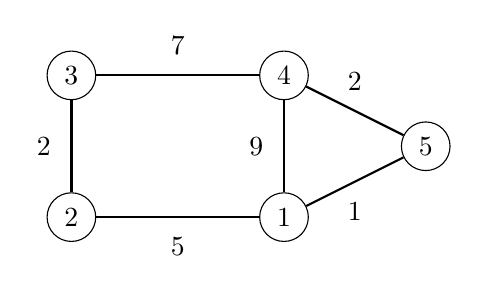
\begin{tikzpicture}[scale=0.9]
        \node[draw, circle] (1) at (1,3) {$3$};
        \node[draw, circle] (2) at (4,3) {$4$};
        \node[draw, circle] (3) at (1,1) {$2$};
        \node[draw, circle] (4) at (4,1) {$1$};
        \node[draw, circle] (5) at (6,2) {$5$};

        \path[draw,thick,-] (1) -- node[font=\small,label=above:7] {} (2);
        \path[draw,thick,-] (1) -- node[font=\small,label=left:2] {} (3);
        \path[draw,thick,-] (3) -- node[font=\small,label=below:5] {} (4);
        \path[draw,thick,-] (2) -- node[font=\small,label=left:9] {} (4);
        \path[draw,thick,-] (2) -- node[font=\small,label=above:2] {} (5);
        \path[draw,thick,-] (4) -- node[font=\small,label=below:1] {} (5);
    \end{tikzpicture}
\end{center}

Inicialmente, la distancia de cada nodo a sí mismo es $0$,
y la distancia entre nodos $a$ y $b$ es $x$ si hay una arista
entre nodos $a$ y $b$ con peso $x$. El resto de distancias son
infinitas.

En este grafo, el arreglo el inicial se ve así:
\begin{center}
    \begin{tabular}{r|rrrrr}
          & 1        & 2        & 3        & 4        & 5        \\
        \hline
        1 & 0        & 5        & $\infty$ & 9        & 1        \\
        2 & 5        & 0        & 2        & $\infty$ & $\infty$ \\
        3 & $\infty$ & 2        & 0        & 7        & $\infty$ \\
        4 & 9        & $\infty$ & 7        & 0        & 2        \\
        5 & 1        & $\infty$ & $\infty$ & 2        & 0        \\
    \end{tabular}
\end{center}
\vspace{10pt}
El algoritmo consiste de rondas consecutivas. En cada ronda, este
elige un nuevo nodo que a partir de ahora puede actuar como nodo
intermedio en caminos, que se utilizan para reducir distancias.

En la primera ronda, el nodo 1 es el nuevo nodo intermedio. Hay un
nuevo camino entre los nodos 2 y 4 con longitud 14, porque el nodo 1
los conecta. También hay un nuevo camino entre los nodos 2 y 5,
con longitud 6.
\begin{center}
    \begin{tabular}{r|rrrrr}
          & 1        & 2           & 3        & 4           & 5          \\
        \hline
        1 & 0        & 5           & $\infty$ & 9           & 1          \\
        2 & 5        & 0           & 2        & \textbf{14} & \textbf{6} \\
        3 & $\infty$ & 2           & 0        & 7           & $\infty$   \\
        4 & 9        & \textbf{14} & 7        & 0           & 2          \\
        5 & 1        & \textbf{6}  & $\infty$ & 2           & 0          \\
    \end{tabular}
\end{center}
\vspace{10pt}

En la segunda ronda, el nodo 2 es el nuevo nodo intermedio.
Esto crea nuevos caminos entre los nodos 1 y 3 y entre los nodos 3 y 5:

\begin{center}
    \begin{tabular}{r|rrrrr}
          & 1          & 2  & 3          & 4  & 5          \\
        \hline
        1 & 0          & 5  & \textbf{7} & 9  & 1          \\
        2 & 5          & 0  & 2          & 14 & 6          \\
        3 & \textbf{7} & 2  & 0          & 7  & \textbf{8} \\
        4 & 9          & 14 & 7          & 0  & 2          \\
        5 & 1          & 6  & \textbf{8} & 2  & 0          \\
    \end{tabular}
\end{center}
\vspace{10pt}

En la tercera ronda, el nodo 3 es el nuevo nodo intermedio. Hay un
nuevo camino entre los nodos 2 y 4:
\begin{center}
    \begin{tabular}{r|rrrrr}
          & 1 & 2          & 3 & 4          & 5 \\
        \hline
        1 & 0 & 5          & 7 & 9          & 1 \\
        2 & 5 & 0          & 2 & \textbf{9} & 6 \\
        3 & 7 & 2          & 0 & 7          & 8 \\
        4 & 9 & \textbf{9} & 7 & 0          & 2 \\
        5 & 1 & 6          & 8 & 2          & 0 \\
    \end{tabular}
\end{center}
\vspace{10pt}

El algoritmo continúa así, hasta que todos los nodos hayan sido
asignados nodos intermedios. Una vez que el algoritmo ha terminado,
el arreglo contiene las distancias mínimas entre cada par de nodos:

\begin{center}
    \begin{tabular}{r|rrrrr}
          & 1 & 2 & 3 & 4 & 5 \\
        \hline
        1 & 0 & 5 & 7 & 3 & 1 \\
        2 & 5 & 0 & 2 & 8 & 6 \\
        3 & 7 & 2 & 0 & 7 & 8 \\
        4 & 3 & 8 & 7 & 0 & 2 \\
        5 & 1 & 6 & 8 & 2 & 0 \\
    \end{tabular}
\end{center}

\newpage
Por ejemplo, el arreglo nos dice que la distancia mínima entre
los nodos 2 y 4 es 8. Esto corresponde al siguiente camino:

\begin{center}
    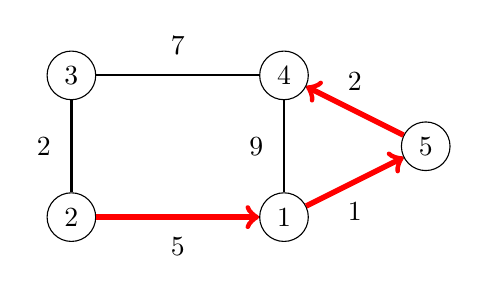
\begin{tikzpicture}[scale=0.9]
        \node[draw, circle] (1) at (1,3) {$3$};
        \node[draw, circle] (2) at (4,3) {$4$};
        \node[draw, circle] (3) at (1,1) {$2$};
        \node[draw, circle] (4) at (4,1) {$1$};
        \node[draw, circle] (5) at (6,2) {$5$};

        \path[draw,thick,-] (1) -- node[font=\small,label=above:7] {} (2);
        \path[draw,thick,-] (1) -- node[font=\small,label=left:2] {} (3);
        \path[draw,thick,-] (3) -- node[font=\small,label=below:5] {} (4);
        \path[draw,thick,-] (2) -- node[font=\small,label=left:9] {} (4);
        \path[draw,thick,-] (2) -- node[font=\small,label=above:2] {} (5);
        \path[draw,thick,-] (4) -- node[font=\small,label=below:1] {} (5);

        \path[draw=red,thick,->,line width=2pt] (3) -- (4);
        \path[draw=red,thick,->,line width=2pt] (4) -- (5);
        \path[draw=red,thick,->,line width=2pt] (5) -- (2);
    \end{tikzpicture}
\end{center}

\subsubsection{Implementación}

La ventaja del algoritmo de Floyd--Warshall es que es fácil de
implementar. El siguiente código construye una matriz de distancias
donde $\texttt{distancia}[a][b]$ es la distancia mínima entre los
nodos $a$ y $b$. Primero, el algoritmo inicializa \texttt{distancia}
usando la matriz de adyacencia \texttt{ady} del grafo:

\begin{lstlisting}
for (int i = 1; i <= n; i++) {
    for (int j = 1; j <= n; j++) {
        if (i == j) distancia[i][j] = 0;
        else if (ady[i][j]) distancia[i][j] = ady[i][j];
        else distancia[i][j] = INF;
    }
}
\end{lstlisting}
Ahora, las distancias mínimas pueden encontrarse de la siguiente manera:
\begin{lstlisting}
for (int k = 1; k <= n; k++) {
    for (int i = 1; i <= n; i++) {
        for (int j = 1; j <= n; j++) {
            distancia[i][j] = min(distancia[i][j],
                                  distancia[i][k] + distancia[k][j]);
        }
    }
}
\end{lstlisting}

La complejidad temporal del algoritmo es $O(n^3)$, porque contiene
tres bucles anidados que visitan todos los nodos del grafo.

Debido a que la implementación del algoritmo de Floyd--Warshall
es simple, puede ser una buena opción incluso si es necesario
encontrar un solo camino mínimo en el grafo. No obstante,
el algoritmo solo es adecuado cuando el grafo es tan pequeño
que una complejidad temporal cúbica es suficientemente rápida.